\documentclass[12pt,a4paper]{article}
\usepackage[utf8]{inputenc}
\usepackage[english]{babel}
\usepackage{amsmath}
\usepackage{amsfonts}
\usepackage{amssymb}


%package for the 1 matrix
\usepackage{dsfont}

%
\usepackage{tikz}
\usetikzlibrary{decorations.markings}

\usepackage{subcaption}

\usepackage{graphicx}
%\usepackage[left=2cm,right=2cm,top=2cm,bottom=2cm]{geometry}
\author{José Antonio García Hernández}
\title{Pure SU(3) lattice gauge theory in equilibrium}
\begin{document}
\maketitle

\section{Introduction}
We study the 4-dimensional SU(3) lattice gauge theory with the compact formulation. In this formulation we consider compact link variables $U_{\mu}(x)\in \text{SU}(3)$ rather than the Lie algebra-valued fields $A_{\mu}(x)$. The compact variables $U_{\mu}(x)$ become the fundamental fields to be integrated over the functional integral. One great advantage of the compact formulation is that we no longer require to fix the gauge.

Link variables are oriented, so they naturally live in the links between neighboring points on the lattice, with spacing $a$. Thus, the variable $U_{\mu}(x)$ is defined in the link between points $x$ and $x + a\hat \mu$ in the positive $\mu$ direction, see Fig.\ \ref{fig:link}. We define the variable between points $x$ and $x + a\hat \mu$ pointing in the negative direction via
\begin{equation}
	U_{-\mu}(x+a\hat\mu) \equiv  U^{\dagger}_{\mu}(x),
\end{equation}
see Fig.\ \ref{fig:conjg_link}.


\begin{figure}
\begin{center}
\begin{subfigure}{0.45\textwidth}
	\begin{center}
	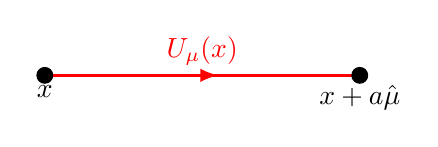
\begin{tikzpicture}
		\tikzset{middlearrow/.style={decoration={markings,mark= at position 0.55 with {\arrow{#1}} ,},postaction={decorate}}};
		\draw[middlearrow={latex}, very thick,red] (0,0)--(4,0);
		\draw[red] (2,0) node[above] {$U_{\mu}(x)$};
		\filldraw[black] (0,0) circle(0.1) node[below]{$x$};
		\filldraw[black] (4,0) circle(0.1) node[below]{$x+a\hat{\mu}$};
	\end{tikzpicture}
	\end{center}
	\caption{Link variable at point $x$ in the $\mu$ direction. $a$ is the lattice spacing.}
	\label{fig:link}
\end{subfigure}
\begin{subfigure}{0.45\textwidth}
	\begin{center}
	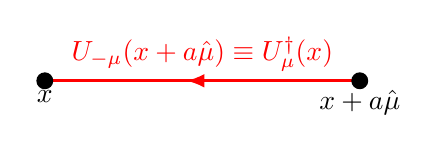
\begin{tikzpicture}
		\tikzset{middlearrow/.style={decoration={markings,mark= at position 0.55 with {\arrow{#1}} ,},postaction={decorate}}};
		\draw[middlearrow={latex}, very thick,red] (4,0)--(0,0);
		\draw[red] (2,0) node[above] {$  U_{-\mu}(x+a\hat\mu) \equiv  U^{\dagger}_{\mu}(x)$};
		\filldraw[black] (0,0) circle(0.1) node[below]{$x$};
		\filldraw[black] (4,0) circle(0.1) node[below]{$x+a\hat{\mu}$};
	\end{tikzpicture}
	\end{center}
	\caption{Link variable at point $x+a\hat\mu$ in the $-\mu$ direction.}
	\label{fig:conjg_link}
\end{subfigure}
\end{center}
\end{figure}

Under a gauge transformation the link variables transform as
\begin{equation}
	U'_{\mu}(x) = \Omega(x) U_{\mu}(x) \Omega^{\dagger}(x+a\hat\mu),
\end{equation}
where $\Omega(x)\in\text{SU}(3)$. We refer to \cite{gattringer} for a complete discussion on lattice gauge theory.



For SU($N$), the lattice gauge action reads
\begin{equation}
	\label{eq:wilson_action}
	S[U] = \frac{\beta}{N}\sum_x \sum_{\mu < \nu} \text{Re}\ \text{Tr} \left[\mathds{1} - U_{\mu\nu}(x) \right],
\end{equation}
where $\beta = \frac{2N}{g^2}$. The plaquettes are defined by
\begin{equation}
	\label{eq:plaquette}
	U_{\mu\nu}(x) = U_{\mu}(x)U_{\nu}(x+\hat{\mu})U_{\mu}^{\dagger}(x+\hat{\nu})U_{\nu}^{\dagger}(x) 
\end{equation}

Sum of plaquette variables
\begin{equation}
	\label{eq:Sp}
	S_{\text{P}} = \frac{1}{N} \sum_x\sum_{\mu < \nu} \text{Re}\ \text{Tr} [U_{\mu\nu}(x)]
\end{equation}
we define
\begin{equation}
	\label{eq:Ep}
	E_{\text{P}} =\frac{ \langle S_{\text{P}} \rangle}{D V}
\end{equation}
where $V=L^d$ is the volume of the lattice and $D = \frac{d(d-1)}{2}$ is the number of planes of rotation.

Staples
\begin{equation}
	\label{eq:staples}
	\Sigma_{\mu}(x) = \sum_{\nu \neq \mu} \left[ U_{\nu}(x)U_{\mu}(x+\hat{\nu})U_{\nu}^{\dagger}(x+\hat{\mu}) + U_{\nu}^{\dagger}(x-\hat{\nu})U_{\mu}(x-\hat{\nu})U_{\nu}(x+\hat{\mu}-\hat{\nu})\right]
\end{equation}


The change in the action  by a local update when changing $U_{\mu}(x) \to U'_{\mu}(x)$ is
\begin{equation}
	\label{eq:DS}
	\Delta S = -\frac{\beta}{N} \text{Re } \text{Tr} \left[ \left( U'_{\mu}(x) - U_{\mu}(x) \right)\Sigma_{\mu}^{\dagger}\right]
\end{equation}


\section{Algorithms}


\section{Results}

\section{Acknowledgements}



\begin{thebibliography}{99}

\bibitem{gattringer} C.\ Gattringer and C.B.\ Lang, \emph{Quantum Chromodynamics on the Lattice: An Introductory Presentation},  Lect.\ Notes Phys.\ 788 (Springer, Berlin Heidelberg 2010).

\bibitem{Metropolis} N.\ Metropolis {\it et al.},
\emph{Equation of State Calculations by Fast Computing Machines},
J.\ Chem.\ Phys.\ {\bf 21} (1953) 1087.

\bibitem{Glauber} R.J.\ Glauber,
  \emph{Time-Dependent Statistics of the Ising Model},
  J.\ Math.\ Phys.\ {\bf 4} (1963) 294.
  
\bibitem{Gerber} U.\ Gerber,
  \emph{Heatbath Algorithm for the 2d U(1) Model}.
  Informal Notes. Universidad Nacional Autónoma de México, 2015.  

\end{thebibliography}

\end{document}